%%
%% 研究報告用スイッチ
%% [techrep]
%%
%% 欧文表記無しのスイッチ(etitle,jkeyword,eabstract,ekeywordは任意)
%% [noauthor]
%%

\documentclass[submit,techrep]{ipsj}
%\documentclass[submit,techrep,noauthor]{ipsj}



\usepackage[dvipdfmx]{graphicx}
\usepackage{latexsym}

\def\Underline{\setbox0\hbox\bgroup\let\\\endUnderline}
\def\endUnderline{\vphantom{y}\egroup\smash{\underline{\box0}}\\}
\def\|{\verb|}
\def\newblock{\hskip .11em plus .33em minus .07em}

\setcounter{巻数}{53}%vol53=2012
\setcounter{号数}{10}
\setcounter{page}{1}

% インタラクション特有の設定。印刷工程で柱・ノンブルの埋め込みを行う。
\makeatletter
\pagestyle{empty}
\def\@oddhead{}%
\def\@evenhead{}%
\def\ps@IPSJTITLEheadings{}
\makeatother

% このソースファイルは,情報処理学会が研究会・シンポジウム用に新しく定め,提供
% している共通テンプレートに対し,インタラクションにおける製版工程の差異上必要と
% なるレイアウト要素について最低限の改変を施したものです.
% インタラクションでは,和文で原稿を作成する場合,タイトル,著者名,アブスト
% ラクト,図表キャプションは日本語で,英文で原稿を作成する場合は英語で記載し,和
% 英の併記はしないで下さい.その他の原稿作成・提出上の注意点は,
% http://www.interaction-ipsj.org/2021/submissions の案内に従ってください.
% 本文は,研究会・シンポジウムの原稿を作成する上での一般的な注意になっています.

\begin{document}


\title{ディスプレイを用いた擬似的脈波生成手法の検討}

\affiliate{RU}{立命館大学}
\affiliate{JST}{JSTさきがけ}

\author{藤井 敦寛}{}{RU}[atsuhiro.fujii@iis.ise.ritsumei.ac.jp]
\author{村尾 和哉}{}{RU,JST}[murao@cs.ritsumei.ac.jp]

\begin{abstract}
	本稿は,情報処理学会論文誌ジャーナルに投稿する原稿を執筆する際,および論
	文採択後に最終原稿を準備する際の注意点等をまとめたものである.大きく分け
	ると,論文投稿の流れと,\LaTeX と専用のスタイルファイルを用いた場合の論
	文フォーマットに関する指針,および論文の内容に関してするべきこと,するべ
	きでないことをまとめたべからずチェックリストからなる.本稿自体も \LaTeX
	と専用のスタイルファイルを用いて執筆されているため,論文執筆の際に参考に
	なれば幸いである.
\end{abstract}

\maketitle

\section{はじめに}
\label{introduction}
近年,健康管理への意識の高まりから,自身の生体情報を記録するウェアラブルデバイスが広く普及している.記録する生体情報は活動量や呼吸数,体温など様々な情報があり,心拍数もその一つである.心拍数を取得するために用いられる脈波センサでは,緑色のLEDを皮膚に照射して,血管を通して反射した光の変化から脈波を計測する光電式容積脈波記録法(PPG)と呼ばれる方式のものが一般的であり,スマートウォッチなどにも導入されている.スマートウォッチのこのセンサから取得できる心拍データを用いて疲労度を検出する手法を今井ら\cite{fatigue_detection}が提案しているなど,脈波センサから得られるデータを使用した研究は盛んである.しかしながら,皮膚内の血管に向けて光を照射するという特性上,センサの装着位置に血管が存在しない場合は使用が不可能である.例えば,義手やロボットアームなどにスマートウォッチを装着する場合,正常な心拍数が取得できない.多くのスマートウォッチは身体活動を記録する機能を持つが,この機能は心拍数データも含めた生体情報から活動状態を識別し,アノテーションを行うものが多い.そのため,正常な心拍数が取得できない場合にはデータにノイズが混入してしまい,正しい活動が記録されない可能性がある.この問題を解決するには,現状では特注のスマートウォッチを別途作成する必要があると考えられる.
\par

本研究では,ディスプレイを用いて擬似的に脈波データを生成する手法を検討する.擬似的に脈波を生成することが可能であれば,スマートウォッチを義手やロボットアームなどに装着する場合でも,任意の脈波を入力することが可能となる.例えば義手装着者の場合,他の身体部位から取得された本人の脈波データを複製し,スマートウォッチに入力することが可能となる.また,ディスプレイを用いるのみでスマートウォッチには手を加えないため,市販のスマートウォッチをそのまま利用することが可能である.本稿は検討段階であるため,あらかじめ収集された実際の脈波データを参考にして,ディスプレイの色調を変化させることで,脈波センサの取得値を意図的に操作する.ディスプレイを用いて擬似的に脈波データを生成することが可能か確認し,提案手法の有効性を明らかにする.
\par

以降,\ref{related}節で関連研究を紹介する.\ref{method}節で提案手法を説明し,\ref{evaluation}節で提案手法の評価実験と結果の考察を行い,最後に\ref{conclude}節で本研究をまとめる.


\section{関連研究}
\label{related}
本節では個人認証手法,身体部位装着型デバイス,頭部状態の認識に関する研究を紹介する.

\subsection{ウェアラブルデバイスの普及}
% ウェアラブルデバイスが普及している
Hamら\cite{smart_wristband}はスマートグラス用の入力デバイスとして,リストバンド型のデバイスを提案している.このデバイスはタッチパネルと慣性計測ユニットを搭載しており,タッチや手首をひねるなどのモーションで操作ができる.手首にデバイスを装着することで使用できるため,ユーザは動きを制限されず,自由度が高い.また,ポインティングにはタッチパネルを使用することで,入力の安定性を向上させた.
Hernandezら\cite{bioglass}は頭部装着型のウェアラブルデバイスである,Google Glassに内蔵された加速度センサ,ジャイロセンサ,カメラから脈拍数と呼吸数を認識する手法を提案している.
Nishajithら\cite{smart_cap}は,視覚障害者の状況認識を支援するウェアラブルデバイスとして,スマートキャップの設計と実装を行った.デバイスはRaspberry Pi 3,Raspberry Pi NoIR Camera V2,イヤホン,電源から構成される.Raspberry Pi NoIR(No Infrared) Camera V2とはRaspberry Piの赤外線カメラモジュールである.この赤外線カメラで得られる画像から検出された対象物について,イヤホンを通して音声で説明する.
これらはいずれも身体部位に装着するウェアラブルデバイスに関する研究であり,さまざまな形状のデバイスを用いた研究が行われている.
\par

さらに,デバイスの装着部位も多岐にわたる.
Vahdatpourら\cite{localization_vahdatpour}は25人の被験者に頭部,胸部,両上腕,両前腕,腰部,両大腿部,両脛部の計10箇所に加速度センサを装着してもらい,日常行動下の加速度データを収集した.収集したデータからSVM(Support Vector Machine)を用いて,平均89\%の精度で装着部位を推定した.
*****Timo ら[12] は15 人の被験者の頭部,胸部,左上腕,左手首,腰部,服の前ポケット,左足首の計7 箇所に加速度センサを装着してもらい,歩行や走るなどの行動の加速度データを収集した.収集したデータからRandom Forest を用いて装着部位を推定し,平均89\%の精度を得ている.Kunze ら[13] は6 人の被験者に右手首,右目の横,ズボンの左ポケット,左胸のポケットに加速度センサを装着してもらい,歩行動作のデータを収集した.収集したデータからC4.5 分類木を用いて装着部位を推定し,平均94\%の精度を得ている.*****
また,筆者ら\cite{localization_yoshida}はウェアラブルデバイスで取得可能な生体情報である心電と脈波を利用し,特定の行動を装着者に行わせることなくウェアラブルデバイスの装着部位を推定する手法を提案している.
\par

このように,ウェアラブルデバイスに関する研究は活発に行われている.


\subsection{脈波データの利用}
また,ウェアラブルデバイスは身体情報を取得するために用いられることが多い.
Spinsanteら\cite{accuracy_in_low_intensity}は低強度の身体活動時にスマートウォッチから取得される心拍数に注目し,その精度を計測している.
Hanら\cite{arrhythmia_detection}は不整脈を検出する手法を提案している.
これらはいずれもウェアラブルデバイスから取得された脈波データを用いた研究であり,正常なデータが取得されているという前提に基づくものである.
\par

一方で我々は,このウェアラブルデバイスに対して入力するデータを擬似的に生成する手法を提案する.

\subsection{脈波センサの制御}
また,澤野さんや秋元のように,脈波センサに入力する手法を提案する研究がある.これらはあくまで人体に装着した場合において,血流を制御することで入力を行う.
一方で本研究は,入力において人体を使用しない.そのため,義手やロボットアームへの利用も可能である.


\section{予備実験}
予備実験として,ディスプレイ上に脈波センサを貼り付けた状態で,ディスプレイの色調を変化させたときの脈波センサの取得値を観察した.

\subsection{実験環境}
参考にする脈波データを事前に収集した.被験者は20代男性1名である.\figref{fig:sensors}の左図に示すように,左手人差し指に光電式容積脈波記録法の脈波センサ(pulsesensor.com製)を装着した.脈波センサはArduinoUNOを介してPCに接続しており,サンプリング周波数は約90Hzで10秒間データの収集を行った.
\par

擬似脈波の生成には,データの収集で使用するPCとは異なるPCのディスプレイを使用した.\figref{fig:sensors}の右図に示すように,ディスプレイ上に脈波センサを乗せ,光が入らないように布で覆った後,ガムテープで固定した.事前に脈波データを取得した時と同じ条件でデータの取得を行った.ディスプレイの色調の変化にはJavaScriptを使用し,ブラウザの背景色を変化させることで制御した.事前に収集した脈波データを1サンプルずつ読み込み,その値に応じた3色で表示を繰り返す.全サンプルの処理が終了した場合,同じデータで再び処理を行う.値が685より大きければR:150, G:19, B:20,465より小さければR:157, G:26, B:27,それ以外の場合はR:156, G:25, B:26の色を表示する.また,色の表示ごとに10[ms]の遅延を挟んだ.

\subsection{結果と考察}
取得された脈波データを,最初のピークから5秒間切り出した結果を\figref{fig:pulse}に示す.結果から,擬似的にピークを生成できていることが確認できる.したがって,ディスプレイを使用するアプローチは有効だといえる.しかしながら,ピークの位置や値に違いが見られる.これは,ディスプレイ制御の開始時刻とセンサ値取得の開始時刻を同期していなかったことや,色の表示ごとの遅延を10[ms]に固定していたことが影響したと考えられる.


\section{まとめと今後}
本研究では,ディスプレイを用いて擬似的に脈波データを生成する手法を実現するために,ディスプレイの色調を変化させることで,脈波センサの取得値を意図的に操作することが可能であるか調査した.今後は,別の身体部位から取得された脈波データをリアルタイムに再現するプログラムを実装する.そのためには,手動ではなく自動でディスプレイの色調を決定し,変化に適応していく必要がある.具体的な実現方法として,ディープラーニングの手法の一つであるLSTM(Long short-term memory)を使用し,直近数秒間のデータを繰り返し入力しながら再現していくことを検討している.


\begin{figure}[!t]
	\begin{center}
		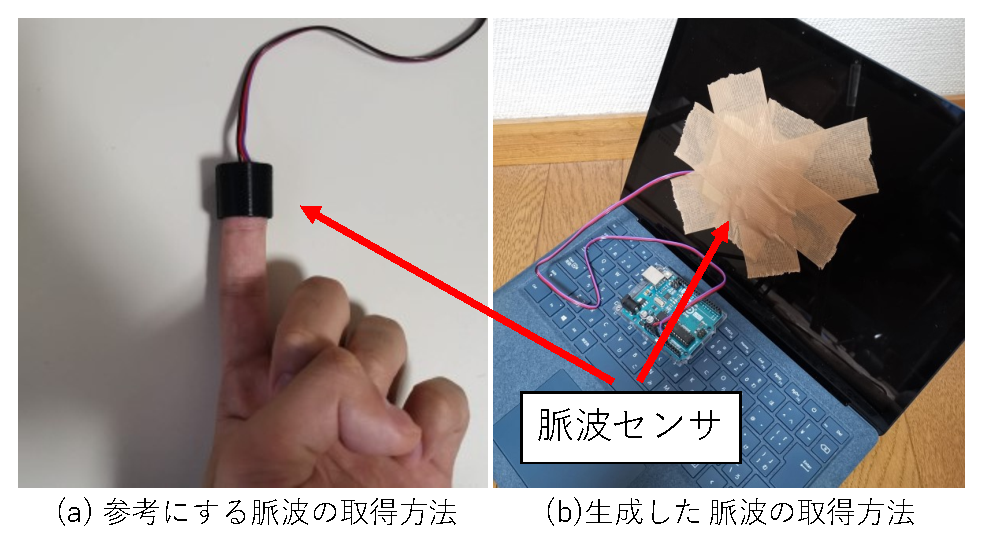
\includegraphics[width=1\linewidth]{sensors.eps}
	\end{center}
	\vspace{-8mm}
	\caption{脈波データの取得方法}
	\label{fig:sensors}
\end{figure}

\begin{figure}[!t]
	\begin{center}
		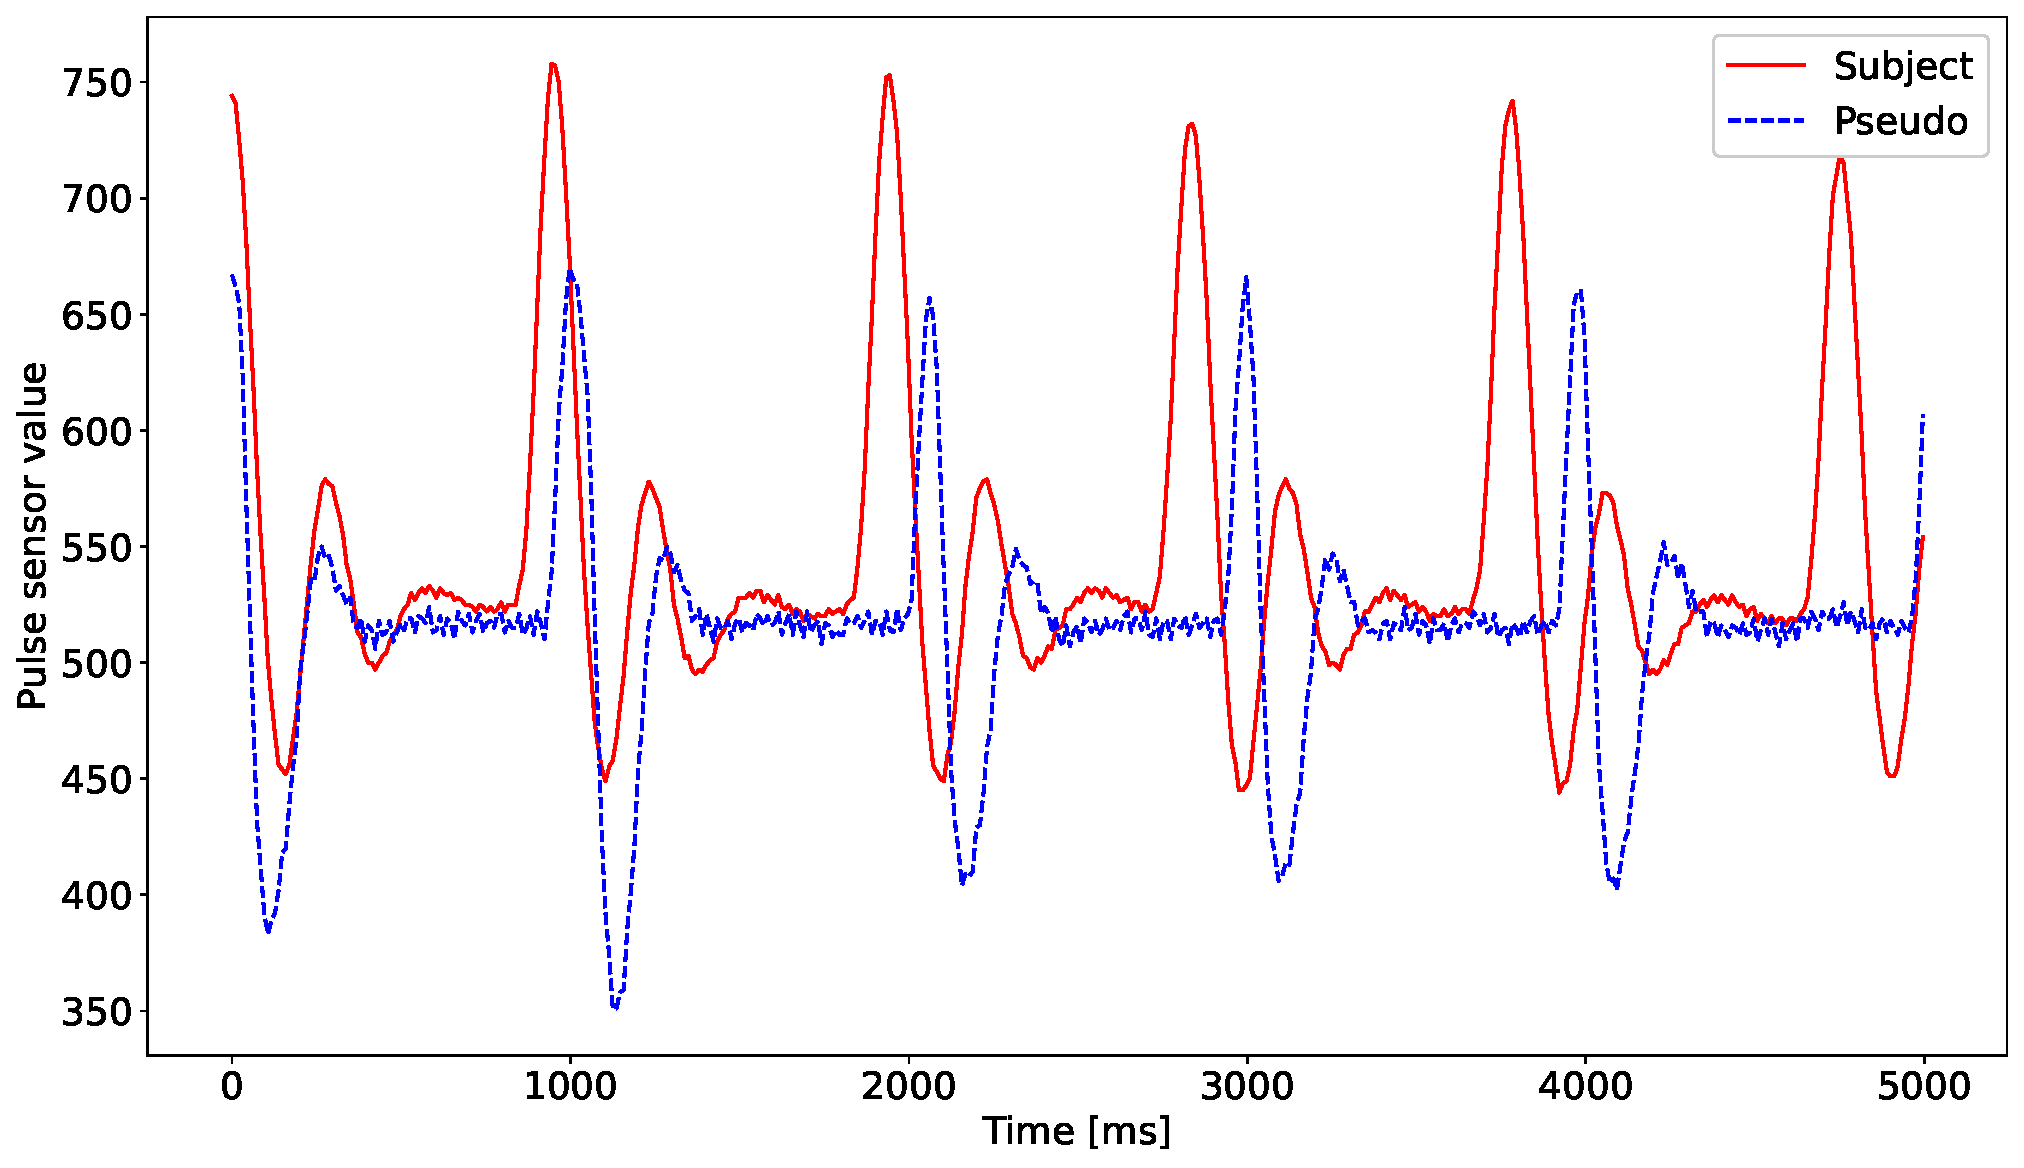
\includegraphics[width=1\linewidth]{pulse.eps}
	\end{center}
	\vspace{-8mm}
	\caption{脈波センサの取得値の変化}
	\label{fig:pulse}
\end{figure}


\bibliography{../../references}
\bibliographystyle{junsrt}

\end{document}
